\begin{figure}[h!]
	\begin{center}
	
	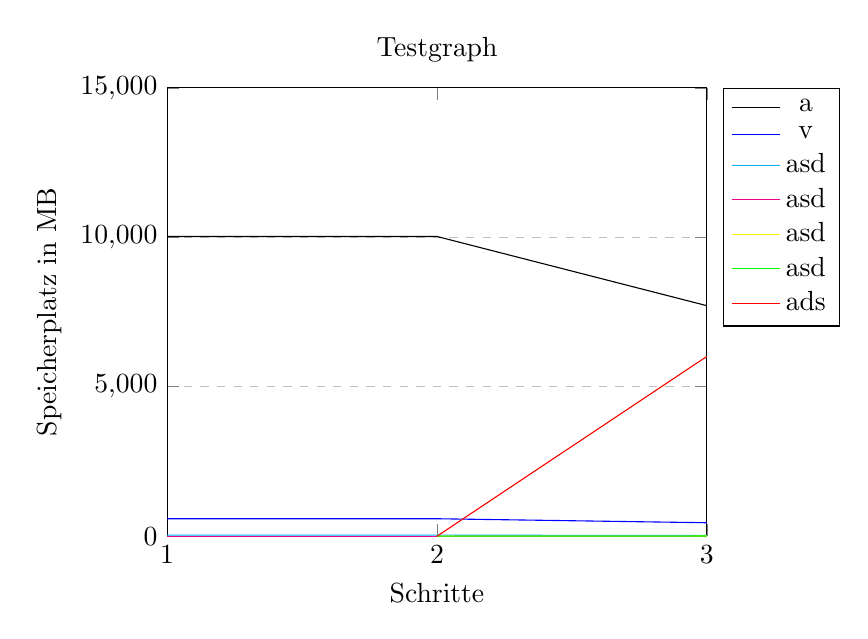
\begin{tikzpicture}
		\pgfplotsset{compat=1.12}
		\begin{axis}[
			title={Testgraph},
			xlabel={Schritte},
			ylabel={Speicherplatz in MB},
			xmin=1, xmax=3,
			ymin=0, ymax=15000,
			xtick={1,2,3},
			ytick={0,5000,10000,15000},
			yticklabel style={
				/pgf/number format/fixed,
				/pgf/number format/precision=5
			},
			scaled y ticks=false,
			legend pos=outer north east,
			ymajorgrids=true,
			grid style=dashed,
			]
			
			\addplot[
				color=black,
				]
				coordinates {
					(1,10028)(2,10028)(3,7713)
				};\label{g-s-1}
			
			\addplot[
			color=blue,
			]
			coordinates {
				(1,584)(2,584)(3,450)
			};\label{g-s-2}
		
			\addplot[
			color=cyan,
			]
			coordinates {
				(1,34)(2,34)(3,23)
			};\label{g-s-3}
		
			\addplot[
			color=magenta,
			]
			coordinates {
				(1,0.02)(2,0.02)(3,0.02)
			};\label{g-s-4}
		
			\addplot[
			color=yellow,
			]
			coordinates {
				(2,0)(3,4.84)
			};\label{g-s-5}
		
			\addplot[
			color=green,
			]
			coordinates {
				(2,0)(3,4.911)
			};\label{g-s-6}
		
			\addplot[
			color=red,
			]
			coordinates {
				(2,0)(3,6013)
			}; \label{g-s-7}
			\addlegendimage{/pgfplots/refstyle=g-s-1}\addlegendentry{a}
			\addlegendimage{/pgfplots/refstyle=g-s-2}\addlegendentry{v}
			\addlegendimage{/pgfplots/refstyle=g-s-3}\addlegendentry{asd}
			\addlegendimage{/pgfplots/refstyle=g-s-4}\addlegendentry{asd}
			\addlegendimage{/pgfplots/refstyle=g-s-5}\addlegendentry{asd}
			\addlegendimage{/pgfplots/refstyle=g-s-6}\addlegendentry{asd}
			\addlegendimage{/pgfplots/refstyle=g-s-7}\addlegendentry{ads}
		\end{axis}
	\end{tikzpicture}
	\end{center}
	\caption{Speicherplatz der Tabellen}
\end{figure}